\begin{figure}[t!]
\centering
  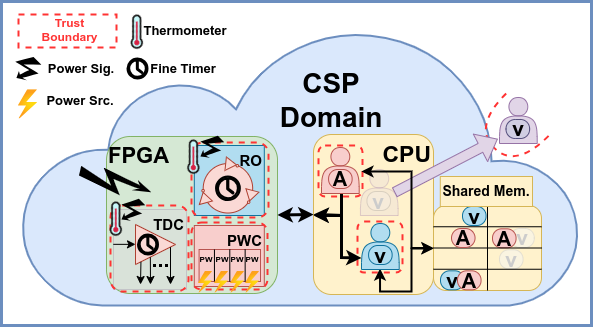
\includegraphics[width=0.9\linewidth]{img/rcs_tm.png}
  \caption{The landscape of RCS threat models. Victim (\textbf{V}) and adversarial (\textbf{A}) tenants perform sensitive operations or attacks, respectively. Both a prior victim and a present victim are shown. The prior victim (purple and shaded regions) is the target of temporal side-channel attacks. The present victim (blue regions) is the target of spatial attacks. Adversarial resources are constructed within the FPGA including time-to-digital converters (\textbf{TDC}), ring oscillators (\textbf{RO}), and power wasting circuits (\textbf{PWCs}). Time-to-digital converters and ring-oscillators can both serve the purpose of fine timing, voltage fluctuation sensing or thermal measurement. Power wasting circuits may be constructed to inject timing faults or a complete failure of the FPGA resource. External power signatures from other processing units or system components may also expose PCB-level side-channels.}
\label{fig:rcs-tm}
\end{figure} 